\documentclass{article}
\usepackage{graphicx,fancyhdr,amsmath,amssymb,amsthm,subfig,url,hyperref,epigraph,lipsum}
\usepackage[margin=1in]{geometry}
\setlength\epigraphwidth{.8\textwidth}

% Bibliography
\usepackage[backend=biber, style=authortitle-comp, refsection=section]{biblatex}
\addbibresource{report.bib}

%----------------------- Macros and Definitions --------------------------

\renewcommand{\theenumi}{\bf \Alph{enumi}}

\fancypagestyle{plain}{}
\pagestyle{fancy}
\fancyhf{}
\fancyhead[RO]{\sffamily\large University of Delhi}
\fancyhead[LO]{\sffamily\large MCS-204 Advanced Computer Networks}
\fancyfoot[RO]{\sffamily\thepage}
\renewcommand{\headrulewidth}{1pt}
\renewcommand{\footrulewidth}{1pt}

\graphicspath{{figures/}}

%-------------------------------- Title ----------------------------------

\title{Emerging Trends in Mobile Communications}
\author{
    Samyak Ahuja \\
    \texttt{Class ID: 29}
    \and
    Mayank Kharbanda \\
    \texttt{Class ID: 16}
}

%--------------------------------- Text ----------------------------------

\begin{document}
\maketitle

\section{Acoustic data transmission}
\epigraph{ I tried to discover, in the rumor of forests and waves, words
that other men could not hear, and I pricked up my ears to listen to the
revelation of their harmony.}{\textcite{november05}}

\subsection{Introduction}
The rise of IoT devices in the home and workplace has created a world where
data and connectivity are becoming increasingly complex. \textcite{ihs16}
predicts a staggering 75 billion connected devices by 2025, up from 26 billion
in 2019, as shown in Figure \ref{fig:ihs_iot}.  As IoT technology advances and the
demand for efficient ways of communicating data between these devices grows,
the world has witnessed a rise in emerging new data transmission technologies
which are looking to provide secure and effective solutions for sharing
information. One solution to meet these rising new demands is “data-over-sound”.

\begin{figure}[!h]
  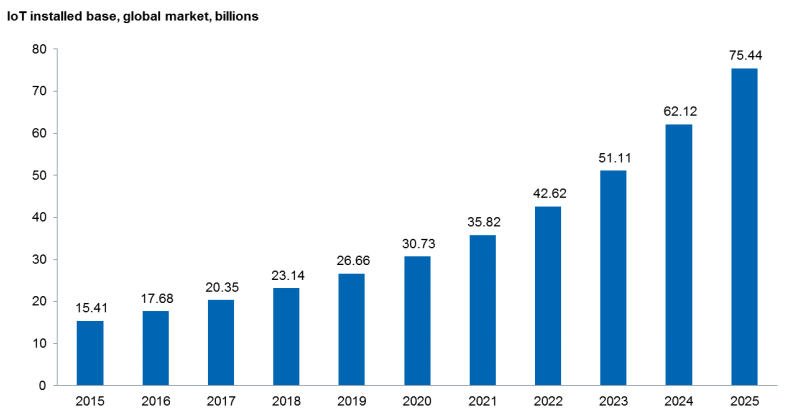
\includegraphics[width=\linewidth]{res/iot_market_trend.png}
    \caption{Number of IOT devices that will be installed worldwide from 2019
    to 2025 (in billions).}
  \label{fig:ihs_iot}
\end{figure}


Data-over-sound (DoS) presents a compelling solution for many device-to-device
connectivity applications, particularly for use cases that require
frictionless, low cost connectivity with nearby devices. DoS harnesses devices’
existing speakers and microphones to send and receive data over an acoustic
channel. Because it doesn’t require any additional networking hardware, DoS has
captured the interest of companies interested in adding wireless connectivity
functionality to existing devices. Some big names such as Google and Cisco
already have point-product DoS integrations

There are a number of connectivity technologies available in the market today,
including extremely short range (NFC and QR); short range, high bandwidth
(Bluetooth and Wi-Fi). Each technology has its advantages which makes it more
or less suitable for certain applications. An overview of these considerations
are given in Table \ref{table:feature_dos}.

\begin{table}[!h]
\begin{center}
\begin{tabular}{r|c|c|c|c|c|c|}
\multicolumn{1}{r}{}
 &  \multicolumn{1}{c}{DoS}
 &  \multicolumn{1}{c}{QR}
 &  \multicolumn{1}{c}{NFC}
 &  \multicolumn{1}{c}{Bluetooth}
 &  \multicolumn{1}{c}{Wi-Fi}
 &  \multicolumn{1}{c}{Li-Fi} \\
\cline{2-7}
    Two-way communication & 1 & 0 & 0 & 1 & 1 & 1 \\
\cline{2-7}
    One-to-many broadcast & 1 & 0 & 0 & 0 & 0 & 1 \\ 
\cline{2-7}
    Non line-of-sight communication & 1 & 0 & 0 & 1 & 1 & 0 \\
\cline{2-7}
    Zero pairing/set-up procedure & 1 & 1 & 1 & 0 & 0 & 0 \\
\cline{2-7}
    Low power operation & 1 & 1 & 1 & 1 & 0 & 0 \\
\cline{2-7}
    max data rate & 1 kb/s & 3 kb & 424 kb/s & 25 mb/s & 70 mb/s & 1 gb/s \\
\cline{2-7}
    max range & 100m & 10:1 & 20/cm & 100/cm & 50m & 10m \\
\cline{2-7}
\end{tabular}
\end{center}
\caption{Feature comparison for DoS vs alternative technologies}
\label{table:feature_dos}
\end{table}

\subsection{Advantages of Data-over-Sound}

According to Table \ref{table:feature_dos} following advantages can be listed.

\begin{description}
    \item [Device interoperability] The simple hardware requirement of a
        speaker and/ or microphone make data-over-sound arguably the most
        wide-reaching wireless communication technology in terms of device
        compatibility. Mobile phones, voice controlled devices, and any device
        with an alarm speaker are able to communicate using data-over-sound.
        This includes many legacy devices. Data can also be transmitted over
        media channels such as radio and TV, and over existing telephone lines.

    \item [Frictionless UX]  Data-over-sound requires no pairing or
        configuration, making data transfer as simple as pressing a button. 

    \item [Physically Bounded]  Because sound waves respect room boundaries,
        particularly in the near-ultrasonic range commonly used in
        data-over-sound, transmissions do not pass between neighbouring rooms.
        This means that it can be used for detecting the presence of a device
        with room-level granularity.

    \item [Zero power] The advent of ‘wake-on-sound’ MEMs microphones such as
        the Vesper VM1010 enables devices to communicate using data-over-sound,
        whilst draining virtually no battery power in between communications ($<$
        10 µA). 
\end{description}

\subsection{Applications of DoS}

Based on these advantages, four key use cases for Chirp (a DoS implementation) are emerging, which are
identified here.

\begin{description}
    \item [IoT device provisioning] Configuring a new smart device with network
        credentials and functional configuration remains a disproportionately
        complex task, particularly for headless devices. Chirp offers an
        approach to provisioning which is offline, locally-bounded, and does
        not require any infrastructure modifications. Credentials are encoded
        as audio, optionally layered with cryptography for secure scenarios,
        and broadcast over-the-air to nearby smart devices. \par
        \begin{minipage}{\linewidth}
            \centering
            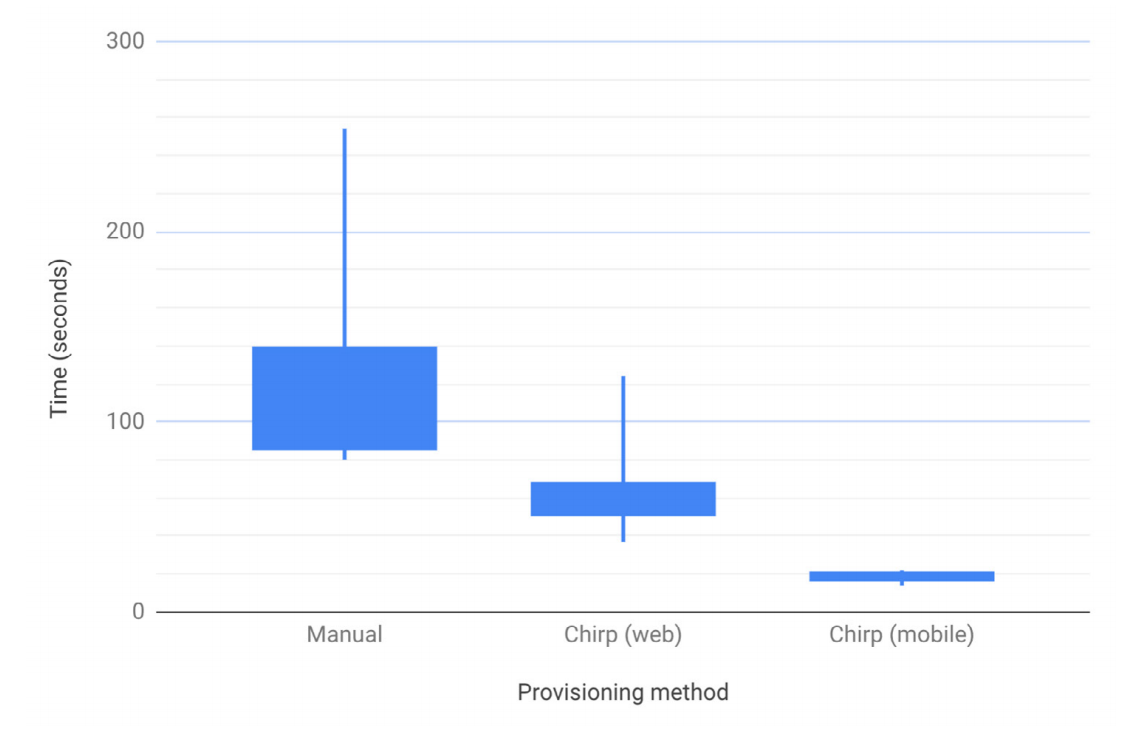
\includegraphics[width=10cm]{res/provisioning_time.png}
            \captionof{figure}{Time taken to provision a smart device.}
            \label{figure:provisioning_time}
        \end{minipage}

        Figure \ref{figure:provisioning_time} shows the result of a study in
        which some experience of IoT were asked to provision a headless smart
        device using three methods: 

        \begin{enumerate}
            \item Manually, by creating a temporary Wi-Fi hotspot on the
                device, connecting to the hotspot with a web browser, and
                entering credentials; 
            \item Using a Chirp-enabled web interface which asks the user to
                enter credentials and transmits them to the device via
                data-over-sound;
            \item Using a Chirp-enabled mobile app which was able to use the
                device’s existing knowledge of the credentials
        \end{enumerate}
        The Chirp-enabled solutions reduced the provisioning time by 48\% with
        the web-based scenario, and 86\% with the mobile scenario.

    \item [Proximity Detection] A key property of acoustic signals is that
        their propagation respects room boundaries, particularly in the
        near-ultrasonic range. As a consequence, there is a growing uptake for
        near-ultrasonic acoustic beacons for presence sensing at room-level
        granularity

    \item [Two way acoustic NFC] Data-over-sound also supports near-field
        communication scenarios whilst offering a two-way full-duplex mode of
        communication, thus addressing a critical limitation of NFC.  Enabling
        two-way data exchange means that devices can perform
        challenge-and-response dialogues - for example, Diffie-Hellman key
        exchange for secure financial transactions, or securely sending
        un-spoofable receipts to a merchant or buyer. 

    \item [Telemetry in RF-restricted environments] In many sensitive
        environments, RF-based communications are prohibited due to the risk of
        sparks or interference with equipment that pre-dates RF regulation.
        Chirp overcomes these limitations, allowing the industrial IoT to
        harness the benefits of wireless communication without limitation.
\end{description}

\subsection{How it all works?}

The basic idea of data-over-sound is no more complex than a traditional
telephone modem.  Data is encoded into an acoustic signal - either audibly as
“bleeps and tones” inaudibly above human hearing range or “hidden” as
imperceptible modifications of existing speech or music - which is then played
through a medium (typically the air, although it could equally be a wired
telephone line or VoIP stream), and received and demodulated by a ‘listening’
device. The listening device then decodes the acoustic signal and returns the
original data. This process is described in Figure \ref{fig:lifecycle_dos}.

\begin{figure}[!h]
  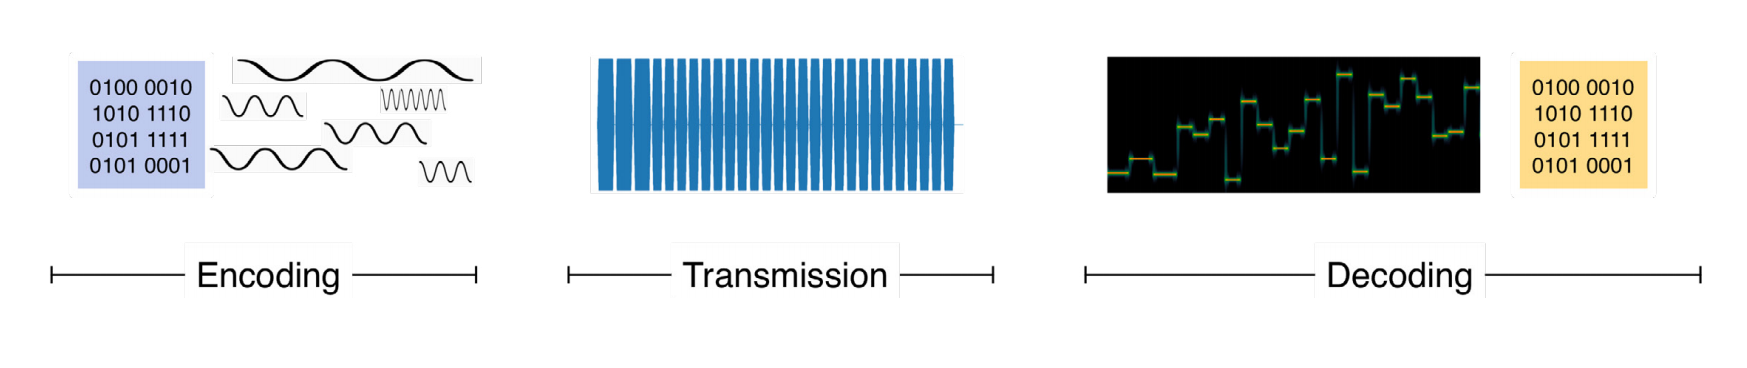
\includegraphics[width=\linewidth]{res/lifecycle_dos.png}
    \caption{life-cycle of data-over-sound}
  \label{fig:lifecycle_dos}
\end{figure}


As with other data transmission protocols, the entire message can include
specific sequences to indicate the start and expected length of a message, as
well as additional bytes for error detection and correction, as shown in Figure
\ref{fig:dos_message}. Messages are typically encoded using frequency-shift
keying (FSK) modulation, which is robust to background noise and distortion
from acoustic effects such as reverberation. Following extensive testing of a
large range of consumer devices, Chirp considers the ‘safe’ range to be between
1kHz-20kHz. This enables the production of audible messages, or near ultrasonic
when limited to ~17kHz-20kHz, which is imperceptible to most adult humans. 

\begin{figure}[!h]
  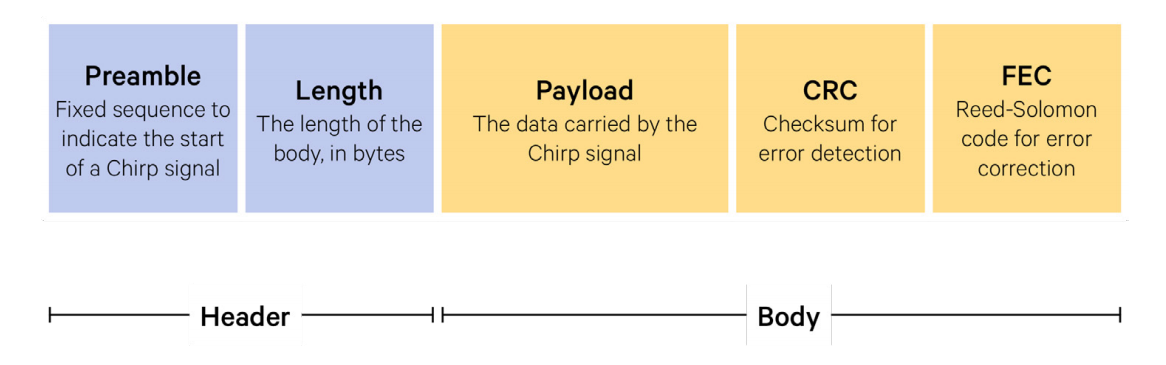
\includegraphics[width=\linewidth]{res/dos_message.png}
    \caption{Makeup of the message}
  \label{fig:dos_message}
\end{figure}

All of Chirp’s standard profiles are tested to perform at \>99\% reliability
under normal operating conditions. Of the existing data-over-sound solutions
on the market, the main differentiator for Chirp is this reliability and
robustness of the internal decoding technology. This has been demonstrated and
stress-tested in acoustically extreme environments, including nuclear power
stations with upwards of 100dB(A) of background noise, across ranges exceeding
100m.

\nocite{chirp17}
\printbibliography[heading=subbibliography]


\vspace{2in}
\section{test}
IGNORE IT. This is a test section to see how final document will look when merged. \\

\lipsum[1-1]
\printbibliography[heading=subbibliography]

\end{document}
